
\begin{enumerate}
    \item A conducting wire of parabolic shape, initially \( y = x^2 \), is moving with velocity \( \vec{V} = V_0 \hat{i} \) in a non-uniform magnetic field \( \vec{B} = B_0 \left( 1 + \left( \frac{y}{L} \right)^\beta \right) \hat{k} \), as shown in figure. If \( V_0 \), \( B_0 \), \( L \) and \( \beta \) are positive constants and \( \Delta \phi \) is the potential difference developed between the ends of the wire, then the correct statement(s) is/are:
        \begin{tasks}(2)
            	\task \( |\Delta \phi| = \frac{1}{2} B_0 V_0 L \) for \( \beta = 0 \)
            	\task \( |\Delta \phi| = \frac{4}{3} B_0 V_0 L \) for \( \beta = 2 \)
            	\task \( |\Delta \phi| \) remains the same if the parabolic wire is replaced by a straight wire, \( y = x \) initially, of length \( \sqrt{2}L \)
            	\task \( |\Delta \phi| \) is proportional to the length of the wire projected on the \( y \)-axis.
        \end{tasks}
\end{enumerate}
\begin{center}
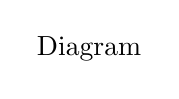
\begin{tikzpicture}
\node {Diagram};
\end{tikzpicture}
\end{center}
